\documentclass[11pt, oneside]{article}
\usepackage{latexrc}
\usepackage{hyperref}

\title{CS3110 Final Project Proposal}
\author{Taeer Bar-Yam (tb442) \and Elizabeth VanDenburgh (eav38) \and Joseph
  Dwyer (jmd456)}
% \date{} % Activate to display a given date or no date

\begin{document}
\maketitle

\section{Status Meeting:}
We will be meeting
\begin{itemize}
\item Tuesdays $18:00-21:00$
\item Thursdays $16:45-18:30$
\item Sundays $12:30-15:00$
\end{itemize}

\section{Proposal:}
Programming an interactive Hnefatafl game.
\subsection{Hnefatafl:}
The game is played on an $11\times 11$ checkered board with two uneven sides.
$12$ white pieces are positioned around a white ``king'' at the center of the
board, with $24$ black pieces arranged on the edges surrounding them.
See~\ref{fig:initial_position}.
\begin{figure}
  \label{fig:initial_position}
  \centering
    \scalebox{.5}{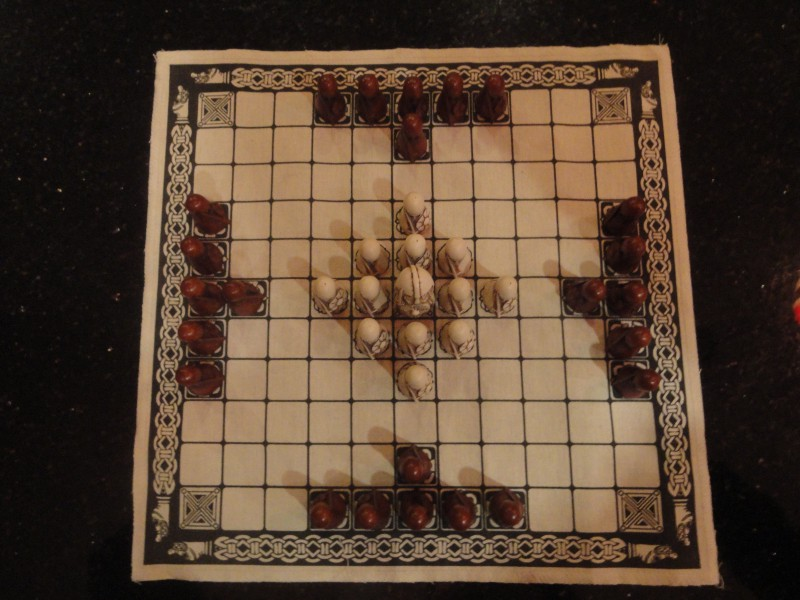
\includegraphics{hnefatafl}}
    \caption{Hnefatafl starting board position. Source: \url{https://medium.com/war-is-boring/you-have-to-play-this-1-600-year-old-viking-war-game-cef088ae4e2d\#.10kof827g}}
\end{figure}
There are three main mechanics involved in the game: 
\begin{enumerate}
\item \textbf{Movement}\\
  All pieces in Hnefatafl except the king move like rooks in chess. That is, $n$
  squares vertically or horizontally in a straight line accross the board, not
  passing any other pieces along the way. The king can only move three squares
  at a time.
\item \textbf{Capturing}\\
  When two pieces of the same color actively flank a piece of the opposite
  color, the flanked piece is removed from the board. Notably this does not
  happen if a piece moves into a position where it is being flanked.
  Additionally, the king cannot participate in flanking. Flanking is defined as
  being surrounded on two opposite sides. In the case of the king it must be
  flanked on all sides.
\item \textbf{Winning}\\
  Black wins when the king is captured, or the king's only escape is to move
  back to the center square of the board.\\
  White wins when the king is moved to one of the side squares of the board.
\end{enumerate}
See: \url{https://en.wikipedia.org/wiki/Tafl\_games\#Hnefatafl}
\subsection{Interface:}
Ultimately we would like to implement the interface as a GUI using openGL, and
allow click-and-drag motion commands. Initially, we will implement a text-based
interface that uses chess-like notation for movement and output a ASCII grid to
show positions of pieces. This interface will likely remain available as an
option\\
This will be playable against another human player, or against an AI.
\subsection{Stretch Goals:}
\begin{itemize}
\item Hnefatafl is an old game, and there are many versions of it that exist.
  Time permitting, we would like to implement many of these variants, working
  off of a general game core.
\item Detect if the game has become unwinable.
\end{itemize}

\end{document}
